\newcommand{\gl}{\mathfrak{gl}}
\newcommand{\lag}{{\mathfrak{g}}}
\newcommand{\ad}{\mathrm{ad}}

\chapter{联络与曲率}
我们已经知道,在惯性参考系中,间隔写作$\dd s^2=c^2 \dd t^2-\dd x^2-\dd y^2-\dd z^2$,如果采用保持惯性参考系的变换,即Lorentz变换,那么间隔不变。可是,如果我们变到了非惯性系,那么间隔一般来说不再能够写作$\dd s^2=c^2 \dd t^2-\dd x^2-\dd y^2-\dd z^2$,比如有一个变换$A$,他不是仿射的,那么$x_2=A(x_1)$后(指标规则依然如同狭义相对论)
\[
	\dd x_2^\mu=\frac{\partial A^\mu}{\partial x_1^\nu}(x_1)\dd x_1^\nu
\]
所以
\[
	(\dd s_2)^2=\eta_{\mu\nu}\dd x_2^\mu\dd x_2^\nu=\eta_{\mu\nu}\frac{\partial A^\mu}{\partial x_1^\rho}(x_1)\frac{\partial A^\nu}{\partial x_1^\sigma}(x_1)\dd x_1^\rho\dd x_1^\sigma,
\]
右边并不能写成$\eta_{\mu\nu}\dd x_1^\mu\dd x_1^\nu$,而是$g_{\mu\nu}\dd x_1^\mu\dd x_1^\nu$,其中
\[
	g_{\rho\sigma}(x_1)=\eta_{\mu\nu}\frac{\partial A^\mu}{\partial x_1^\rho}(x_1)\frac{\partial A^\nu}{\partial x_1^\sigma}(x_1)
\]
不再是对角的,而且也不再是一个常矩阵。

Einstein认为,非惯性参考系中产生的动力学效应可以等价为一个力场的作用(当然,这个力场和真的力场还是有些许不同的),从上面可以看到,这个力场应当完全由时空的几何结构(度规)决定。此外,Einstein认为,真实存在的重力场也应该是时空的几何结构的改变,同样被度规决定。所以,时空的几何结构不再是时空的固有性质,不再是一切物理现象的背景,而本身参与到物理过程中,本身是一种物理对象。

这就是史上第一个非Abel场论,即广义相对论的一些基本想法。已经看到,前面所谈论的狭义相对论的基本背景是平直空间,比如$\rr^4$或者$\rr^{3+1}$,但现在我们必须扩展到流形上,为此伪Riemann几何是必须的,假设大家已经知道了一些流形上的微积分。

下面的讨论建立在伪Riemann流形(Semi-Riemannian Manifold)上,首先给出他的定义。

\begin{defi}
假设$M$是一个可微流形,且在他每一点的切空间$T_pM$都存在度规,即一个非退化\footnote{即如果$\langle a,a\rangle=0$,则$a=0$.}的对称二重线性映射$\langle\star,\star\rangle_p:T_pM\times T_pM\to \rr$.

由于二重线性映射可以看作一个2-形式$g_p:T_pM\times T_pM\to \rr$,因此度规可以看出一个2-形式场$g$。局部来看
\[
	g_p(u,v)=u^iv^jg(e_i,e_j)=u^iv^jg_{ij},
\]
最后的要求,$(g_{ij})$的负本征值的个数不变\footnote{根据惯性定理,负本征值的个数和选取的基无关。},即如果在一点为$I$个,其他点都是$I$个。这样的$(M,g)$就被称为一个伪Riemann流形。当$I=0$时候,就变成Riemann流形。
\end{defi}

因为$(g_{ij})$对实对称矩阵,所以可以对角化成实对角矩阵,所以非退化条件等价于没有零本征值或者
$\det (g_{ij})\neq 0$。

前面我们已经在$\rr^4$上选取了度规$\eta$使得$\rr^4$变成了一个伪Riemann流形$\rr^{3+1}$,但是这样的说法还是有些模糊。之所以我们能说是在$\rr^4$上选取了度规,是因为$\rr^4$在每一点的切空间$T_p\rr^4$都同构于$\rr^4$,并且,在每一点定义的内积,都可以看作全局定义的在$\rr^4$上定义的度规。但是到了可微流形上,就必须强调这些区别。

指标规则基本不变,但以后不再用英文字母表示空间部分,而是指任意需要累加的指标。

$g^{il}$是$g_{il}$的逆,更准确地说就是$g^{il}g_{lm}=\delta^i_m$.

抬升和下降指标依然由度规$g$完成,即$x_i=g_{ij}x^j$和$x^i=g^{ij}x_j$,需要注意的是,现在求导和提升或者下降指标不再对易,因为$g$是可以改变的。
\section{测地线}
在伪Riemann流形上可以使用度规来定义可微曲线$\gamma:[a,b]\to M$的长度
\[
	L(\gamma)=\int_a^b \sqrt{|\langle\gamma'(\tau),\gamma'(\tau)\rangle|}\dd \tau=\int_a^b \sqrt{|g(\gamma'(\tau),\gamma'(\tau))|}\dd \tau.
\]
如果在物理上理解一条$\gamma$为一个粒子的世界线,则还要加上$\langle\gamma'(\tau),\gamma'(\tau)\rangle>0$的假设,此时$L(\gamma)$就是世界线的线长,其中参数$\tau$不一定有什么物理意义。类比在$\rr^{3+1}$里面解耦合的作用量的形式\eqref{freeparticle},可以定义作用量积分为
\[
	S(\gamma)=-\frac{mc}{2}\int_a^b \langle\gamma'(\tau),\gamma'(\tau)\rangle\dd \tau,
\]
而使得$S(\gamma)$取极值的路径被称为测地线。

为了求出测地线,将作用量积分在局部坐标下面写出来,用$x$来表示从$M$到$\rr^n$的局部平凡化,就是说$x(\tau)=x(\gamma(\tau))$是$\rr^n$中的坐标,此外用$\dot{f}$来表示$\dd f/\dd \tau$,则
\[
	S(\gamma)=-\frac{mc}{2}\int_a^b g_{ij}(x(\tau))\dot{x}^i(\tau)\dot{x}^j(\tau)\dd \tau,
\]
他的Lagrange方程直接计算后,发现可以写作
\[
	\ddot{x}^i(\tau)+\Gamma^i_{\phantom{i}jk}(x(\tau))\dot{x}^j(\tau)\dot{x}^k(\tau)=0,
\]
其中
\[
	\Gamma^i_{\phantom{i}jk}=\frac{1}{2}g^{il}(\partial_k g_{jl}+\partial_j g_{kl}-\partial_l g_{jk})
\]
被称为Christoffel记号,下面我们讨论联络的时候还会再遇到。如果有了上述方程的一个解$x(\tau)$,下面将要指出的是$\langle\dot{x}(\tau),\dot{x}(\tau)\rangle$是一个常数,就像我们在狭义相对论里面说的$u^\mu u_\mu=1$一样。这点直接计算
\[
	\frac{\dd}{\dd \tau}\langle\dot{x}(\tau),\dot{x}(\tau)\rangle=\frac{\dd}{\dd \tau}\left(g_{ij}(x(\tau))\dot{x}^i(\tau)\dot{x}^j(\tau)\right)=0
\]
就可以了,其中要用到上面的Lagrange方程。这个结论可以理解成测地线的切矢量的模长$\langle\gamma',\gamma'\rangle$是一个常数。

测地线局部的存在唯一性靠着二阶常微分方程的理论就可以得到,从局部到整个空间,我们可以一个一个坐标卡延拓过去,但是否可行这里不做讨论。

在参数化过程中,选取一个有意义的参数有利于我们观察问题,这里,如同狭义相对论里面一样,可以采用线元来参数化我们的曲线,这个时候
\[
	L(\gamma)=\int \sqrt{|\langle\gamma'(s),\gamma'(s)\rangle|}\dd s=\int_a^b \sqrt{|g(\gamma'(s),\gamma'(s))|}\dd s,
\]
将$u=\gamma'(s)$看成速度矢量,可以类比定义动量$p=mcu$.又注意到$\langle u,u\rangle$在选取$s$作为参数的时候满足(不怎么严格,但是用其他方法强行算一波还是有下面这个结论)
\[
	(\dd s)^2\langle u, u\rangle=g_{ij}\frac{\dd x^i}{\dd s}\frac{\dd x^j}{\dd s}(\dd s)^2=g_{ij}\dd x^i\dd x^j=(\dd s)^2,
\]
所以$\langle u, u\rangle=1$,因此
\[
	p^ip_i=g_{ij}p^i p^j=m^2c^2.
\]

反过来,假如粒子的运动轨迹是测地线,此时在线元参数化下$\langle u,u\rangle=u^iu_i=1$构成一个约束,我们可以检查作用量依然可以写作
\[
	S=-mc \int \dd s
\]
的形式,检查的过程和相对论力学那节中的几乎一模一样。但是第一要注意在$u^i u_i=g_{ij}(x) u^i u^j$不再不显含$x$了,此外
\[
	0=\frac{\dd}{\dd s}\left(g_{ij}u^iu^j\right)=u^j\frac{\dd}{\dd s}\left(g_{ij}u^i\right)+g_{ij}u^i(u^j)'=u^i(u_i)'+u_i(u^i)',
\]
所以我们不能草率地说$u$和$\dd u /\dd s$是相互正交的矢量。

只要注意上面两点,运动方程写作
\[
	l_i=(2(u_i)'-\partial_ig_{mn}u^mu^n)\lambda+2u_i \lambda',
\]
记$2k_i=2(u_i)'-\partial_ig_{mn}u^mu^n$,只要存在一个和$k_i$正交但不和$u_i$正交的矢量$v^i$,这样
\[
	l_iv^i=2v^iu_i \lambda',
\]
只要满足$l_iv^i=0$就自然有$\lambda'=0$.这是我们最感兴趣的情况,因为这种情况下,作用量的自由粒子部分可以看作
\[
	S=-\frac{mc}{2}\int_a^b g_{ij}u^i u^j \dd s.
\]
而整个运动方程就写成
\[
	l_i=-mck_i=-\frac{mc}{2}\left(2(u_i)'-\partial_ig_{mn}u^mu^n\right).
\]

\section{矢量丛及其联络}

联络的出现,代数上实现了对矢量场的方向导数,几何上实现了所谓的平行移动。讨论联络的基本背景是矢量场和主丛,他们都是纤维丛的一个特例。

\begin{defi}纤维丛:一个纤维丛$(E,\pi,M,F)$是指,$E$, $M$和$F$都是可微流形,投影$\pi:E\to M$可微,对于每一个$x\in E$,在$\pi(x)$的附近可以找到一个邻域$U$使得存在一个微分同胚$\varphi$满足下列交换图:
\begin{figure}[htp]
	\centering
	\[
		\xymatrix{
			\pi^{-1}\left(U\right)\ar[rr]^\varphi \ar[dr]_\pi&&U\times F \ar[dl]^{\mathrm{proj}_1}\\
			&U&
			}
	\]
	\caption{Locally Trivialition}
\end{figure}

其中$M$被称为底空间,而$F$被称为纤维。值得注意的是,因为有局部平凡化,所以对每一点$p\in M$都成立$\pi^{-1}(p)\cong F$.
\end{defi}
如果一个丛的纤维是矢量空间\footnote{当然一个实数域上的$n$维矢量空间都同构于$\rr^n$,看作$\rr^n$不失一般性。},这个丛就被称为矢量丛,所以纤维是张量空间,就被称为张量丛。

\begin{defi}截面:
一个纤维丛$(E,\pi,M,F)$的光滑截面$s$就是一个光滑函数$s:M\to E$满足$\pi\circ s=\mathrm{Id}_E$.所有光滑截面的集合我们记作$\Gamma(E)$.
\end{defi}
因为在每一点,$s(p)\in \pi^{-1}(p)\cong F$,所以$s(p)$可以看成是$F$中的元素。就是说,一个光滑截面,在流形$M$的每一点都赋予一个$s(p)\in F$,这就是我们熟知的场的概念的推广。

显然$E=M\times F$是一个平凡的纤维丛,就干脆称为平凡丛,他的截面可以如图做出来:
\begin{figure}[htbp]
\centering
	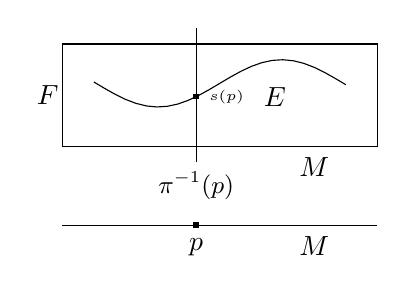
\begin{tikzpicture}[scale=1]
		\draw (-2,-0.3)--(2,-0.3)--(2,1)--(-2,1)--cycle;
		\node [label=left:$F$] (F) at (-1.8,0.35) {};
		\node [label=below:$M$] (M1) at (1.2,-0.2) {};
		\node [label=below:$M$] (M2) at (1.2,-1.2) {};
		\node [label=below:$E$] (E) at (0.7,0.7) {};
		\draw (-2,-1.3)--(2,-1.3);
		\node [fill=black, inner sep=1pt, label=below:$p$] (p) at (-0.3,-1.3) {};
		\draw [color=black, domain=-1.6:1.6] plot (\x,{0.3*sin(2*\x r)+0.5});
		%0.5-0.3*sin(0.6)=0.330607...
		\node [fill=black, inner sep=1pt, label=right:\tiny$s(p)$] (s) at (-0.3,0.3306) {};
		\draw (-0.3,-0.5)node[below]{\small$\pi^{-1}(p)$}--(-0.3,1.2);
	\end{tikzpicture}
	\caption{Trivial Bundle and its Section}
\end{figure}

一个矢量丛的重要例子就是切丛,他是流形每一点切空间的不交并
\[
	TM =\coprod_{x\in M}T_xM=\bigcup_{x\in M} \left\{x\right\}\times T_xM
	=\bigcup_{x\in M} \left\{(x, y)\vert\; y\in T_xM\right\},
\]
他有自然的投影$\pi : TM \rightarrow M $使得$\pi(x, v) = x$. 这个投影将一点的切空间$T_pM$映到了点$p$上.同样地,余切丛、张量丛都可以这么定义。

矢量场是矢量丛的截面,特别地,度规是2-形式场(形式是余切矢量),局部来看就是
\[
	g=g_{ij}(x)\dd x^i\otimes \dd x^j.
\]

矢量丛上的联络的首先目的是为了对矢量场进行求导的。按照一般的思路,将矢量场$s$参数化,假设他在曲线$\gamma(t)$上,$\gamma(0)=x_0$,而$\gamma'(0)=Y$,则似乎他沿$Y$方向的导数应该定义成
\[
	\lim_{t\to 0}\frac{s(\gamma(t))-s(x_0)}{t},
\]
可是$s(\gamma(t))$和$s(x_0)$属于不同点的切空间,不能相减。在$\rr^n$很容易克服这个困难,只要将两个切空间的矢量的端点平移到一起,这样就可以相减了。但是到了流形上,就会发现没那么简单,最简单的问题,什么是平移?下面我们先抽象地定义联络,然后再回来说这个问题。

\begin{defi}
令$E$是一个矢量丛,一个(线性)联络或者说一个协变导数是指一个映射
\[
	D:\Gamma (E)\to\Gamma(E)\otimes \Gamma(T^*M)
\]
满足下面几条规则:记$Ds(V)=D_Vs$,则$D_V:\Gamma (E)\to\Gamma(E)$,对于任意的$V,W\in T_p M$, $r,s\in \Gamma (E)$和$f,g\in C^\infty(M,\rr)$满足
\[
\begin{array}{lcl} 
	D_{fV+gW}s &=& fD_Vs+gD_W s,\\
	D_V(r+s)   &=& D_Vr+D_Vs,\\
	D_V(fs)    &=& (Vf)s+fD_Vs.
\end{array}
\]
\end{defi}

$T\rr^n$的截面可以写作$s(x)=x^i(x)e_i$,其中$e_i$是$\rr^n$的标准基,此时
\[
	D_Vs=\dd x^i(V) e_i=(Vx^i)e_i,
\]
是一个联络。

任何一个截面局部都可以写成$s=s^i\mu_i$,其中矢量场$\mu_i$对应着矢量空间的一组基,而对于切矢量来说,局部可以写作$X=X^i\partial_i$,所以
\[
	D_Xs=X^iD_{\partial_i}(s^j\mu_j)=X^i\partial_i s^j\mu_j+X^is^jD_{\partial_i}\mu_j=X(s^j)\mu_j+X^is^jD_{\partial_i}\mu_j,
\]
由于$D_{\partial_i}\mu_j$依然是一个截面,所以他是$\mu_i$的线性组合
\[
	D_{\partial_i}\mu_j=\Gamma^k_{\phantom{k}ij}\mu_k,
\]
其中$\Gamma^k_{\phantom{k}ij}$被称为Christoffel符号,以后会看到,前面出现过的Christoffel符号只是这里的特例。此外,以后在局部用$D_i$来记$D_{\partial_i}$.综上,联络在局部可以写作
\[
	D_Xs=X(s^j)\mu_j+X^is^j\Gamma^{k}_{ij}\mu_k.
\]

有了联络的概念,我们可以谈什么叫做平行移动,假设现在我们有一条可微曲线$c(t)$,那么他的切矢量是$\dot{c}(c(t))$,或者在局部写作$\dot{c}^k(t)\partial_k$,对于任意的$M$上的截面$s$可以计算沿着这个曲线切线的导数
\begin{align*}
	D_{\dot{c}}s(c(t))&=\dot{c}^k(t)\partial_ks^j\mu_j(c(t))+(\dot{c}^i s^j\Gamma^k_{\phantom{k}ij}\mu_k)(c(t))\\
	&=\left(\dot{s}^j\mu_j+\dot{c}^i s^j\Gamma^k_{\phantom{k}ij}\mu_k\right)(c(t)).
\end{align*}
\begin{defi}
	如果$c(t)$是$M$上一条可微曲线,则称满足$D_{\dot{c}(t)}s(t)=0$的解$s(t)$是$s(0)$在$E$中沿着曲线$c$的平行移动。
\end{defi}

由于$\dot{s}^j\mu_j+\dot{c}^i s^j\Gamma^{k}_{ij}\mu_k=0$是系数$\dot{s}^j$的一阶常微分方程组,所以解出系数后,就解出了$s$,即给定一个初值$s(0)$,有唯一解$s(t)$满足上述方程。

现在来检查联络是如何和平行移动联系起来的。对于$M$上的两个点,找一条曲线$c(t)$连接两点,且在一点处的切矢量为$Y$,假设有一组联络的基$\mu_i(t)$他们沿着$c(t)$平行,即$D_{\dot{c}(t)}\mu_i(t)=0$,定义$P_{c,t}(s(t))$将$s(t)$平行移动回$s(0)$,局部来看就是
\[
	P_{c,t}(s^i(t)\mu_i(t))=s^i(t)\mu_i(0).
\]
此时按照联络的定义,可以计算得到$D_{\dot{c}(t)}s(t)=\dot{s}^i(t)\mu_i(t)$,
令$t\to 0$,则
\[
	D_{Y}s(0)=\lim_{t\to 0}\frac{s^i(t)\mu_i(0)-s^i(0)\mu_i(0)}{t}=\lim_{t\to 0}\frac{P_{c,t}(s(t))-s(0)}{t},
\]
这正是我们前面希望得到的矢量场沿一个方向的导数的定义。

现在解释“联络”的意思,假如有一个矢量丛$E$,他的切丛为$TE$,在每一点$p=(\pi(p),v)$,$T_pE$都有一个确定的子空间,即每一点纤维的切空间$T_vE_p$,所谓的联络就是在每一点选定了$T_pE$中$T_vE_p$的补空间\footnote{补空间不唯一,所以需要选定,比如在$\rr^3$中,一条直线的补空间可以是任意不和他平行的平面。}$H_p$,即选定了$H_p$使得$T_pE=T_vE_p\oplus H_p$。$T_vE_p$被称为垂直子空间,或记做$V_p$,而$H_p$则被称为水平子空间,这个命名的直观可以考察平凡丛$E=M\times F$,$T_vE_p=T_v F$是切于$F$的,而$F$可以看做和$M$垂直。垂直子空间的不交并构成一个矢量丛,我们称为垂直丛,他是原本矢量丛的子丛,同样我们有水平丛。

一旦有了一个联络,任意$M$中的一条曲线$c(t)$都可以将$\dot{c}(0)=X$通过平行移动得到$E$中的一条曲线$\psi(t)$。对于同一个$X$,可以考察不同曲线$c(t)$平行移动后得到的切矢量们$\dot{\psi}(0)$,他们构成$T_{(c(0),X)}E=T_{s(0)}E$的一个子空间,这就是$H_{\psi(0)}$.因为$\psi(t)$是使用$D$平行移动而成,他在纤维上的投影是$P_{c,t}^{-1}s(0)$,因此他的切矢量在垂直子空间上的投影$\mathrm{p_v}(\dot{\psi}(0))$是
\[
	\mathrm{p_v}(\dot{\psi}(0))=\lim_{t\to 0}\frac{P_{c,t}^{-1}s(0)-s(0)}{t}
	=-\lim_{t\to 0}P_{c,t}^{-1}D_{X}s(0)=0,
\]
因此$\dot{\psi}(0)\in H_{\psi(0)}$.

上面这种看法可以看做联络的一种定义,因为他是Ehresmann首先形式化定义的,所以也被称为Ehresmann联络。使用Ehresmann联络,可以比较方便对联络的存在性等问题进行考察,也方便搞清楚平行移动的直观等等,详细而严谨的讨论可以参看Jeffrey M. Lee的\emph{Manifolds and Differential Geometry}一书中的第12章。

重新观察
\[
	D_Xs=X(s^j)\mu_j+s^jX^i\Gamma^{k}_{ij}\mu_k=\dd s^j(X)\mu_j+s^jX^i\Gamma^k_{\phantom{k}ij}\mu_k,
\]
将$X^i\Gamma^{k}_{ij}\mu_k$写作$A(X)\mu_j$,那么就可以写出$D=\dd +A$或者更细致一些
\[
	D(s)=D(s^i\mu_i)=\dd s^i \mu_i+s^i A\mu_i.
\]
特别地,对于基$\mu_i$,$D\mu_i=A\mu_i$.现在来看看$A$到底是什么东西,由于$A(X):\mu_j \mapsto X^i\Gamma^k_{\phantom{k}ij}\mu_k=\dd x^i(X)\Gamma^k_{\phantom{k}ij}\mu_k$,或者将$A(X)$写成矩阵
\[
	A_{\phantom{j}i}^{j}(X)=\Gamma^j_{\phantom{j}ki}\dd x^k(X)
\]
因此$A$不是别的,而是一个1-形式值的矩阵,写形式一点$A\in \Gamma(\mathfrak{gl}(n,\rr)\otimes T^*M|_U)$,其中下标$U$指我们在局部考虑这个问题。以后将$A$称为联络$D$的联络形式。

局部来看矢量从$E$,设$U_\alpha$是$M$的一个坐标图册,那么丛的局部平凡化给出了$\varphi_\alpha:\pi^{-1}(U_\alpha):U_\alpha\to U_\alpha\times V$。这样,在非空的$U_\alpha\cap U_\beta$上,我们对于$E$的同一点$p$就有了按$\varphi_\alpha$和$\varphi_\beta$不同的平凡化,他们之间靠一个转移函数$\varphi_{\beta\alpha}:U_\alpha\cap U_\beta\to \gl(V)$相互联系,即
\[
	\varphi_\beta\circ \varphi_\alpha (x,v)=(x,\varphi_{\beta\alpha}(v)),
\]
这个式子也可以直接看做转移函数的定义。

对于同一处不同局部化的同一个截面$s$,我们使用转移函数将其联系起来$s_\beta=\varphi_{\beta\alpha}s_\alpha$,这样,对于局部来看的联络$D_\alpha=\dd+A_\alpha$和$D_\beta=\dd+A_\beta$就有
\[
	\varphi_{\beta\alpha}D_\alpha s_\alpha=D_\beta s_\beta=D_\beta (\varphi_{\beta\alpha}s_\alpha),
\]
具体写出来
\[
\begin{array}{llcl}
	&\varphi_{\beta\alpha}\dd s_\alpha+\varphi_{\beta\alpha}A_\alpha s_\alpha&=&\dd(\varphi_{\beta\alpha}s_\alpha)+A_\beta(\varphi_{\beta\alpha}s_\alpha)\\
	\Rightarrow &\varphi_{\beta\alpha}A_\alpha s_\alpha&=&\dd(\varphi_{\beta\alpha})s_\alpha+A_\beta(\varphi_{\beta\alpha}s_\alpha)\\
	\Rightarrow &A_\alpha &=&\varphi_{\beta\alpha}^{-1}\dd\varphi_{\beta\alpha}+\varphi_{\beta\alpha}^{-1}A_\beta \varphi_{\beta\alpha}.
\end{array}
\]
所以联络形式并不像一个张量一样变化,但是两个不同联络形式的差却是,所以两个联络的差是一个张量场。

一个矢量丛的对偶丛就是指纤维相互为对偶空间的丛,对偶丛上当然也会有联络,因为他也是一个矢量丛。对偶丛上的光滑截面取值为对偶矢量,因此,对偶丛上的光滑截面和矢量丛上的光滑截面在每点通过内积给出了一个值,这就是说$(\mu,\nu^*)$是$M$上的一个光滑实函数,因此我们可以对其求外微分,而两个丛的联络可以通过类似于Leibniz法则通过内积相互联系,即
\[
	\dd (\mu,\nu^*)=(D\mu,\nu^*)+(\mu,D^*\nu^*),
\]
左边右边都是1-形式,所以定义是合理的,这样,通过丛上的联络$D$就定义了对偶丛上的对偶联络$D^*$.令$\mu_j$是局部的一组基,则$(\mu_i,\mu^j)=\delta_{i}^j$且
\[
	0=\dd(\mu_i,\mu^j)=(A^k_{\phantom{k}i}\mu_k,\mu^j)+(\mu_i, A_{k}^{*j}\mu^k)=A^j_{\phantom{j}i}+A_{i}^{*j},
\]
即$A^*=-A^T$,其中上标$T$表示转置。如果用Christoffel符号表示对偶联络,则$D^*_{i}\mu^j=\mu^k\Gamma_{ki}^{\phantom{ki}j}$,两个系数的关系是
\[
	\Gamma_{\phantom{k}ij}^{k}=-\Gamma_{ji}^{\phantom{ji}k}
\]

\begin{defi}
矢量丛$E_1$和$E_2$的张量积$E_1\otimes E_2$指底空间$M$不变,而纤维变成原本纤维们的张量积。设在$E_1$和$E_2$上有联络$D_1$和$D_2$,则在$E$上按如下方法定义了一个联络$D$
\[
	D(s_1\otimes s_2)=D_1s_1\otimes  s_2+s_1\otimes D_2s_2.
\]
\end{defi}

一个有趣的空间是$\mathrm{End}(E)=E\otimes E^*$,令$\sigma=\sigma^{i}_{\phantom{i}j}\mu_i\otimes \mu^j$是$\mathrm{End}(E)$的一个截面,则
\begin{align*}
	D\sigma&=\dd \sigma^{i}_{\phantom{i}j} \mu_i\otimes \mu^j+\sigma^{i}_{\phantom{i}j}D\mu_i\otimes \mu^j+\sigma^{i}_{\phantom{i}j}\mu_i\otimes D^*\mu^j\\
	&=\dd \sigma+A_{\phantom{k}i}^{k}\sigma^{i}_{\phantom{i}j}\mu_k\otimes \mu^j+\sigma^{i}_{\phantom{i}j}\mu_i\otimes A_{k}^{*j}\mu^k\\
	&=\dd \sigma+A_{\phantom{k}i}^{k}\sigma^{i}_{\phantom{i}j}\mu_k\otimes \mu^j-\sigma^{i}_{\phantom{i}j}A_{\phantom{j}k}^{j}\mu_i\otimes\mu^k\\
	&=\dd \sigma+[A,\sigma].
\end{align*}

类似的计算可以给出任意张量场$\omega$的联络满足:
\begin{pro}假如$\omega$是一个$(r,s)$型张量场,则
\begin{align*}
	X(\omega(\eta^i;X_j))=&(D_X\omega)(\eta^i;X_j)\\
	&+\sum_i \omega\left(\eta^{1},\cdots,\eta^{i-1},D^*_X \eta^i,\eta^{i+1},\cdots,\eta^r;X_j\right)\\
	&+\sum_j \omega\left(\eta^i;X_{1},\cdots,X_{j-1},D_X X_j,X_{j+1},\cdots,X_s\right).
\end{align*}
\end{pro}
这个等式可以理解成广义的Leibniz法则。
\section{曲率}
前面已经知道
\[
	D:\Gamma (E)\to\Gamma(E)\otimes \Gamma(T^*M)=\Gamma(E)\otimes \Omega^1(M),
\]
其中$\Omega^1(M)$是1-形式场,$\Gamma(E)\otimes \Omega^1(M)$中的元素可以看做矢量值的1-形式,那么自然,可以将$\Gamma(E)\otimes \Omega^p(M)$看做矢量值的$p$-形式,不妨将其记做$\Omega^p(E)$,以及$\Gamma (E)=\Omega^0 (E)$,则联络实际上是完成了矢量值的$0$-形式到矢量值的$1$-形式的转变:
\[
	D:\Omega^0 (E)\to \Omega^1(E).
\]
类似于$\dd$是从$p$-形式到$(p+1)$-形式的转变,我们希望拓展联络完成$\Omega^p (E)$到$\Omega^{p+1}(E)$的转变。

首先定义一个$s$-形式$\omega_1$和一个矢量值的$r$-形式$\sigma=\mu\otimes\omega_2\in \Omega^r (E)$的楔积,自然
\[
	\sigma\wedge \omega_1=\mu\otimes(\omega_2\wedge \omega_1)
\]
就构造出了一个矢量值的$(r+s)$-形式。然后我们扩展联络如下:对一个矢量值的$r$-形式$\sigma=\mu \otimes \omega$,其中$\omega$是一个$r$-形式,定义
\[
	D\sigma=D\mu \wedge\omega+\mu\otimes \dd \omega.
\]

但是,正如我们熟知的恒等式$\dd^2=0$,他其实在局部是等价于等式$\partial_i \partial_j=\partial_j \partial_i$,或者$[\partial_i,\partial_j]=0$,直观上就是说,沿着正交方向先后求导,他们的结果是一样的。前面已经看到了,$\rr^n$上存在联络$D=\dd$,因此在$\rr^n$上的这个联络依然是满足$D^2=0$的。可以指出,$[\partial_i,\partial_j]=0$是因为我们是在同一个切空间内求导的结果,而这就忽略掉了流形本身的具体结构,而联络并不会。

为了更清晰地看到这一点,设$s=s^i\mu_i$,计算
\begin{align*}
	D^2 s&=D(\dd s^i \mu_i+s^iA\mu_i)\\
	&=D\mu_i\wedge \dd s^i+D(s^i A^{j}_{\phantom{j}i}\mu_j)\\
	&=A\mu_i\wedge \dd s^i+D(s^i\mu_j)\wedge A^{j}_{\phantom{j}i}+s^i\mu_j\dd A^{j}_{\phantom{j}i}\\
	&=-\dd s^i\wedge A\mu_i+D(s^i\mu_j)\wedge A^{j}_{\phantom{j}i}+(\dd A)s\\
	&=s^i A\mu_j\wedge A^{j}_{\phantom{j}i}+(\dd A)s\\
	&=s^i \mu_k A^{k}_{\phantom{k}j}\wedge A^{j}_{\phantom{j}i}+(\dd A)s\\
	&=(A\wedge A)s+(\dd A)s.
\end{align*}
所以作用在矢量值0-形式上,$D^2=A\wedge A+\dd A$,这个量,我们另外给个名字。
\begin{defi}
一个联络$D$的曲率为
\[
	F:=D^2:\Omega^0(E)\to \Omega^2(E).
\]
\end{defi}
根据上面求的,局部曲率算符有$F=A\wedge A+\dd A$,他一般来说不为0,如果曲率算符为0,则称这个联络是平坦的。

曲率算符可以看做$\mathrm{End}(E)$值的2-形式,因为$F:\Omega^0(E)\to \Omega^2(E)$,于是
\[
	F\in \Omega^2(E)\otimes (\Omega^0(E))^*=\Gamma(E)\otimes \Omega^2(M)\otimes \Gamma(E^*)=\Gamma(\mathrm{End}(E))\otimes \Omega^2(M),
\]
这就是说$F\in \Omega^2(\mathrm{End}(E))$.

设$A=A_i\dd x^i$,其中$A_i$是$n\times n$矩阵,直接计算给出了
\[
	F=\frac{1}{2}\left(\partial_{[i}A_{j]}+[A_i,A_j]\right)\dd x^i\wedge \dd x^j.
\]
观察这个式子是很有趣的,前面在电磁学里面定义了电磁场张量$F_{ij}=\partial_{[i}A_{j]}$,其中$A_i$是四维势。如果四维势对应联络形式,那么电磁场张量对应着曲率。曲率中多出来的$[A_i,A_j]$在电磁学中是自然消失的。

直接的计算可以给出:
\begin{theo}Bianchi等式:
\[
	DF=0.
\]
\end{theo}

使用$A_\alpha=\varphi_{\beta\alpha}^{-1}\dd\varphi_{\beta\alpha}+\varphi_{\beta\alpha}^{-1}A_\beta \varphi_{\beta\alpha}$,我们考察$F$在坐标变换下的改变
\begin{align*}
	F_\alpha&=A_\alpha\wedge A_\alpha+\dd A_\alpha\\
	&=\varphi_{\beta\alpha}^{-1}A_\beta \wedge A_\beta \varphi_{\beta\alpha}+ \varphi_{\beta\alpha}^{-1}A_\beta \varphi_{\beta\alpha}\wedge \varphi_{\beta\alpha}^{-1}\dd\varphi_{\beta\alpha}+\varphi_{\beta\alpha}^{-1}\dd\varphi_{\beta\alpha}\wedge \varphi_{\beta\alpha}^{-1}A_\beta \varphi_{\beta\alpha}+\dd A_\alpha\\
	&=\varphi_{\beta\alpha}^{-1}A_\beta \wedge A_\beta \varphi_{\beta\alpha}+ \varphi_{\beta\alpha}^{-1}A_\beta \wedge \dd\varphi_{\beta\alpha}-\dd\varphi_{\beta\alpha}^{-1}\varphi_{\beta\alpha}\wedge \varphi_{\beta\alpha}^{-1}A_\beta \varphi_{\beta\alpha}+\dd A_\alpha\\
	&=\varphi_{\beta\alpha}^{-1}A_\beta \wedge A_\beta \varphi_{\beta\alpha}+ \varphi_{\beta\alpha}^{-1}A_\beta \wedge \dd\varphi_{\beta\alpha}-\dd\varphi_{\beta\alpha}^{-1}\wedge A_\beta \varphi_{\beta\alpha}+\dd A_\alpha\\
	&=\varphi_{\beta\alpha}^{-1}A_\beta \wedge A_\beta \varphi_{\beta\alpha}+ \varphi_{\beta\alpha}^{-1}A_\beta \wedge \dd\varphi_{\beta\alpha}+\varphi_{\beta\alpha}^{-1}\dd \left(A_\beta \varphi_{\beta\alpha}\right)\\
	&=\varphi_{\beta\alpha}^{-1}A_\beta \wedge A_\beta \varphi_{\beta\alpha}+\varphi_{\beta\alpha}^{-1}(\dd A_\beta)\varphi_{\beta\alpha}\\
	&=\varphi_{\beta\alpha}^{-1}F_\beta \varphi_{\beta\alpha}.
\end{align*}
在计算过程中,使用了
\[
	0=\dd I=\dd (\varphi_{\beta\alpha}^{-1}\varphi_{\beta\alpha})=\dd \varphi_{\beta\alpha}^{-1}\varphi_{\beta\alpha}+\varphi_{\beta\alpha}^{-1}\dd\varphi_{\beta\alpha},
\]
所以$F$变换得符合张量的变换方式,即$F$是一个张量。可以将$Fs$写作$R(\star,\star)s$,其中$R$被称为曲率张量,下面的定理实现了用联络表示曲率张量$R$,证明依然是直接的计算。
\begin{theo}一个联络$D$的曲率张量$R$满足
	\[
		R(X,Y)s=D_XD_Ys-D_YD_Xs-D_{[X,Y]}s.
	\]
\end{theo}
因为他是张量,所以
\[
	R(X,Y)(fs)=fR(X,Y)s,
\]
此外对$X,Y$都函数线性从上面的定理来看是显然的,还有$R(X,Y)+R(Y,X)=0$也是显然的。

前面提到了,曲率涉及了流形本身(包含联络)的具体结构,从曲率张量来看,给定一个光滑曲线族$f(s,t):\rr\times \rr\to M$,按照曲线$f(s,0)$将切矢量$v$从$f(0,0)$平行移动到$f(1,0)$,然后按照曲线$f(1,t)$平行移动到$f(1,1)$,之后平行移动到$f(0,1)$,最后平行移动回$f(0,0)$得到了新的切矢量$v'$,曲率就是度量了$v'$和$v$之间的差异。

\section{Levi-Civita联络}
将上面两节的理论应用到伪Riemann流形,应用到伪Riemann流形的切丛上。切丛上的联络不用$D$而写作$\nabla$.

由于伪Riemann流形的切丛上赋予了度规,这就比前面单纯的矢量场上的联络理论要有更多内容,这一点体现在联络和度规相容条件上:
\[
	\dd \langle \mu,\nu\rangle=\langle \nabla\mu,\nu\rangle+\langle\mu,\nabla\nu\rangle.
\]
或者
\[
	X \langle \mu,\nu\rangle=\langle \nabla_X\mu,\nu\rangle+\langle\mu,\nabla_X\nu\rangle.
\]

当然Levi-Civita联络要比这还要特殊一点。切丛上除了曲率,还能定义一个叫做挠率的张量
\[
	T(X,Y)=\nabla_X Y-\nabla_Y X-[X,Y].
\]
Levi-Civita联络的挠率为0,即Levi-Civita联络是无挠的。联络无挠在局部等价于$\Gamma^{k}_{\phantom{k}ij}=\Gamma^{k}_{\phantom{k}ji}$. 挠率的几何意义其实并不很清楚。

\begin{theo}
伪Riemann流形存在唯一的和度规相容的、无挠的联络,我们称之为Levi-Civita联络。
\end{theo}
\begin{proof}
唯一性的证明,和度规相容的、无挠的联络$\nabla$一定满足:
\[
	\langle \nabla_XY,Z\rangle=\frac{1}{2}\left(X\langle Y,Z\rangle+Y\langle X,Z\rangle-Z\langle X,Y\rangle+\langle[X,Y],Z\rangle-\langle[X,Z],Y\rangle-\langle[Y,Z],X\rangle\right).
\]

利用和度规相容
\begin{align*}
	X\langle Y,Z\rangle&=\langle \nabla_XY,Z\rangle+\langle Y,\nabla_XZ\rangle,\\
	Y\langle X,Z\rangle&=\langle \nabla_YX,Z\rangle+\langle X,\nabla_YZ\rangle,\\
	Z\langle X,Y\rangle&=\langle \nabla_ZX,Y\rangle+\langle X,\nabla_ZY\rangle.
\end{align*}
利用无挠性$\nabla_X Y-\nabla_Y X=[X,Y]$,则
\[
	X\langle Y,Z\rangle+Y\langle X,Z\rangle-Z\langle X,Y\rangle=2\langle \nabla_XY,Z\rangle-\langle[X,Y],Z\rangle+\langle[X,Z],Y\rangle+\langle[Y,Z],X\rangle.
\]
唯一性证明完毕。

存在性的证明,固定$X,Y$,令右边的为$\omega(Z)$,则可以直接计算得$\omega(fZ)=f\omega(Z)$,此外$\omega(Z_1+Z_2)=\omega(Z_1)+\omega(Z_2)$。那么从度规的非退化可以得知,存在唯一的$A$使得
\[
	\langle A,Z\rangle=\omega(Z),
\]
这样子,令$\nabla_XY=A$,最后检验这是一个无挠、和度规相容的联络即可。
\end{proof}

伪Riemann流形的Levi-Civita联络的Christoffel记号为
\[
	\Gamma^i_{\phantom{i}jk}=\frac{1}{2}g^{il}(\partial_k g_{jl}+\partial_j g_{kl}-\partial_l g_{jk}),
\]
注意到,这就是前面我们里面作用量求测地线方程时候出现的Christoffel记号。

\begin{defi}
设有切丛上的联络$\nabla$,则一条可微曲线$c(t)$称为自平行的或者称为测地线,如果其满足$\nabla_{\dot{c}}\dot{c}=0$.
\end{defi}
利用
\[
D_{\dot{c}}s(c(t))=\left(\dot{s}^j\mu_j+\dot{c}^i s^j\Gamma^k_{\phantom{k}ij}\mu_k\right)(c(t)),
\]
直接给出测地线方程为
\[
\nabla_{\dot{c}}\dot{c}=\ddot{c}^j\mu_j+\dot{c}^i \dot{c}^j\Gamma^k_{\phantom{k}ij}\mu_k=0,
\]
再简单一些
\[
\ddot{c}^k+\dot{c}^i \dot{c}^j\Gamma^k_{\phantom{k}ij}=0.
\]

很久以前,在谈论作用量原理的时候,讲到要寻找和$k_i$正交的矢量$v^i$,其中
\[
	2k_i=2(u_i)'-\partial_ig_{mn}u^mu^n,
\]
现在我们指出$k_i=(\nabla_{u}u)_i$,所以寻找和$k_i$正交的矢量$v^i$就是指寻找一个矢量场$v$使得
\[
	\langle \nabla_{u}u,v\rangle=0.
\]
利用Levi-Civita联络的性质
\[
	u\langle u,u\rangle=2\langle \nabla_{u}u,u\rangle.
\]
因为$\langle u,u\rangle=1$,所以$v=u$就是一个自然的解,这和狭义相对论里面讨论的一样。如果使用联络的记号,那么在$l_iu^i=0$情况下粒子的运动方程写作
\[
	l_i=-mc(\nabla_{u}u)_i=-(\nabla_{u}p)_i.
\]

本节的最后来谈谈活动标架法,活动标架法利用的是局部基和对偶基来计算联络和曲率。从直接的计算开始,可以得到:
\begin{pro}
设$D$是无挠联络,则
\[
	\dd \omega(X_1,\cdots,X_{r+1})=\sum_{i=1}^{r+1}(-1)^{i-1}D_{X_i}\omega(X_1,\cdots,\hat{X_i},\cdots,X_{r+1}),
\]
其中$\hat{X_i}$指在括号中没有这项。
\end{pro}

对$r=1$和Levi-Civita联络,
\[
	\dd \omega(X,Y)=\nabla^*_{X}\omega(Y)-\nabla^*_{Y}\omega(X),
\]
对$\mu^i$使用上式,注意到$\nabla^*\mu^i=A^*\mu^i=\mu^jA^{*i}_j=-\mu^jA^i_{\phantom{i}j}$,得到
\begin{align*}
	\dd \mu^i(X,Y)=\nabla^*_{X}\mu^i(Y)-\nabla^*_{Y}\mu^i(X)&=-\mu^j(Y)A^i_{\phantom{i}j}(X)+\mu^j(X)A^i_{\phantom{i}j}(Y)\\
	&=(\mu^j\otimes A^i_{\phantom{i}j}-A^i_{\phantom{i}j}\otimes \mu^j)(X,Y)\\
	&=(\mu^j\wedge A^i_{\phantom{i}j})(X,Y),
\end{align*}
所以
\begin{equation}
	\dd \mu^i=\mu^j\wedge A^i_{\phantom{i}j}=-A^i_{\phantom{i}j}\wedge \mu^j,
	\label{cartan1}
\end{equation}
交换后有负号是因为这是两个1-形式。

前面已经对$s=s^i\mu_i$算过
\[
	F s=s^i \mu_k A^{k}_{\phantom{k}j}\wedge A^{j}_{\phantom{j}i}+s^i\mu_j\dd A^{j}_{\phantom{j}i},
\]
对$s=\mu_i$有
\[
	F \mu_i=\mu_k A^{k}_{\phantom{k}j}\wedge A^{j}_{\phantom{j}i}+\mu_j\dd A^{j}_{\phantom{j}i},
\]
所以
\[
	R(X,Y) \mu_i=F \mu_i(X,Y)=\mu_k A^{k}_{\phantom{k}j}\wedge A^{j}_{\phantom{j}i}(X,Y)+\mu_j\dd A^{j}_{\phantom{j}i}(X,Y),
\]
另一方面将$R(X,Y)$写成分量的形式
\[
	R(X,Y) \mu_k=X^iY^jR_{ijk}^{\phantom{ijk}l}\mu_l=R_{ijk}^{\phantom{ijk}l} \mu^i\otimes\mu^j(X,Y)\mu_l=\frac{1}{2}R_{ijk}^{\phantom{ijk}l} \mu^i\wedge\mu^j(X,Y)\mu_l
\]
其中$R_{ijk}^{\phantom{ijk}l}=\mu^l(R(\mu_i,\mu_j)\mu_k)$,最后一个等号使用了$R(X,Y)$关于$X$, $Y$是反对称的,所以$R_{ijk}^{\phantom{ijk}l}$中的$i$, $j$也是反对称的,于是
\begin{equation}
	\frac{1}{2}R_{mni}^{\phantom{mni}k} \mu^m\wedge\mu^n=A^{k}_{\phantom{k}j}\wedge A^{j}_{\phantom{j}i}+\dd A^{k}_{\phantom{k}i}.
	\label{cartan2}
\end{equation}

式\eqref{cartan1}和\eqref{cartan2}统称Cartan结构方程。有时候会记
\[
	\Omega^{k}_{\phantom{k}i}=-\frac{1}{2}R_{mni}^{\phantom{mni}k} \mu^m\wedge\mu^n,
\]
称之为曲率形式,那么结构方程写作
\[
	\dd A^{k}_{\phantom{k}i}=-\Omega^{k}_{\phantom{k}i}-A^{k}_{\phantom{k}j}\wedge A^{j}_{\phantom{j}i}.
\]

从一般的曲率张量本身可以构造几个特殊的曲率,比如
\begin{defi}
设$\Pi$为切空间$T_pM$的二维子空间,取他的一组基$X$, $Y$,定义$\Pi$的截面曲率为
\[
	K(\Pi)=\frac{\langle R(X,Y)X,Y\rangle}{\langle X,X\rangle\langle Y,Y \rangle-\langle X,Y \rangle^2}.
\]
容易直接计算验证$K(\Pi)$的定义和基的选取无关。
\end{defi}
\begin{defi}
取$X,Y,Z\in T_p M$,那么映射$X\to R(Y,X)Z$就是一个$T_p M$上的自同态,定义这个自同态的迹
\[
	\mathrm{Ric}(Y,Z)=\tr (X\to R(Y,X)Z)
\]
为Ricci曲率张量。他直接出现在Einstein场方程中。
\end{defi}
\section{Hodge星算子}
假设流形是可定向的无边流形\footnote{Hodge用一套整体分析的方法来研究了de Rham上同调群,而他的星算子就是这套方法中很重要的一个部分。稍稍具体一点,Hodge通过在Riemann流形上引入度量,利用度量在每一个同调类中选出代表元,而每个代表元都是椭圆算子的核,然后就可以使用椭圆算子核的性质。具体的展开这里不可能表。},此外下面谈到的形式都是有紧支集的。所以根据Stokes定理,$(n-1)$-形式的外微分在整个流形上的积分为0.

从体积形式开始,在流形的局部,比如考虑$(U,\phi)$,上面的度规有$g_{ij}$,同样地,$(U',\phi')$和$g'_{ij}$,现在假设两个局部是相交的,则体积形式作为几何量,应该是不变的。设在$U$上的坐标为$x$,$U'$上的为$y$,所以
\[
	\mathrm{d}y^1\wedge \cdots \wedge\mathrm{d}y^n=\det\left(\frac{\partial y}{\partial x}\right)\mathrm{d}x^1\wedge \cdots \wedge \mathrm{d}x^n,
\]
其中$\partial y/\partial x$是坐标变换的Jacobian,这里选取的坐标变换是保向的,即Jacobian的行列式大于零。

体积形式必然同时正比于$\mathrm{d}y^1\wedge \cdots \wedge \mathrm{d}y^n$和$\mathrm{d}x^1\wedge \cdots \wedge \mathrm{d}x^n$,当然这是不够的,他还依赖于度规的选取。我们考虑一下度规的变化
\[
	g_{ij}'=g(\partial_i',\partial_j')=g\left(\frac{\partial x^k}{\partial y^i}\partial_k,\frac{\partial x^l}{\partial y^j}\partial_l\right)=\frac{\partial x^k}{\partial y^i}\frac{\partial x^l}{\partial y^j}g_{kl},
\]
为了消掉上面那个行列式,我们考虑一下上式的行列式
\[
	\det(g_{ij}')=\det\left(\frac{\partial x}{\partial y}\right)^2\det(g_{ij})=\det\left(\frac{\partial y}{\partial x}\right)^{-2}\det(g_{ij})
\]
这里出现了2,所以还要开方一下,则有
\[
	\sqrt{|\det(g_{ij}')|}=\det\left(\frac{\partial y}{\partial x}\right)^{-1}\sqrt{|\det(g_{ij})|}
\]
综上
\[
	\sqrt{|\det(g_{ij}')|}\mathrm{d}y^1\wedge \cdots \wedge \mathrm{d}y^n=\sqrt{|\det(g_{ij})|}\mathrm{d}x^1\wedge \cdots \wedge \mathrm{d}x^n,
\]
这是一个几何量,因此他就是体积形式。

Hodge星算子的定义和第一章里面的一样
\[
	\omega\wedge(\star \mu)=\langle \omega,\mu\rangle \mathrm{vol},
\]
通过耐心细致但不复杂的计算可以得到,
\begin{pro}
在伪Riemann流形$M$上,如果他的度规的负本征值个数为$s$,那么在$p$-形式上成立恒等式
	\[\star\star=(-1)^{s+p(n-p)}.\]
\end{pro}
证明很类似在$\rr^{s+(n-s)}$上的证明。

有了Hodge星算子,可以在任意两个$p$-形式之间定义一个新的内积
\[
	(\omega,\mu)=\int \omega\wedge(\star \mu),
\]
很容易看出他是双线性的。

现在假如有一个$(p-1)$形式$\omega$,那么对任意的$p$-形式$\mu$,$(\dd \omega,\mu)$是可以定义的,这样,类似于定义转置算符,我们可以定义$\dd$的对偶算子$\dd^\star$如下
\[
	(\omega,\dd^\star\mu)=(\dd \omega,\mu).
\]
所以$\dd^\star$完成的是从$p$形式到$(p-1)$-形式的转变,只是是否存在还尚且未知。

对$\omega\wedge\star\mu$求外微分
\begin{align*}
	\dd (\omega\wedge\star\mu)&=\dd \omega\wedge\star\mu+(-1)^{p-1}\omega\wedge\dd(\star\mu)\\
	&=\dd \omega\wedge\star\mu+(-1)^{p-1}\omega\wedge\dd(\star\mu)\\
	&=\dd \omega\wedge\star\mu+(-1)^{p-1}(-1)^{s+(p-1)(n-p+1)}\omega\wedge\star\star\dd(\star\mu)\\
	&=\dd \omega\wedge\star\mu-(-1)^{s+(p+1)n+1}\omega\wedge\star(\star\dd\star\mu),
\end{align*}
两边积分后,左边由Stokes公式直接为0,所以
\[
	0=(\dd \omega,\mu)-(-1)^{s+(p+1)n+1}(\omega,\star\dd\star\mu),
\]
最后就求得了
\[
	\dd^\star=(-1)^{s+(p+1)n+1}\star\dd\star.
\]
所以前面写过的含源部分的Maxwell方程组$\star\dd \star \mathbf{F}=-4\pi\mathbf{j}$就等价于
\[
	\dd^\star \mathbf{F}=-4\pi\mathbf{j}.
\]

\begin{defi}
Hodge-Laplace算子定义如下:
\[
	\Delta=\dd^\star\dd+\dd\dd^\star.
\]
他将$p$-形式变成$p$-形式。
\end{defi}
他的一些性质直接计算即可,比如$\Delta\star=\star\Delta$.他是Laplace算子在流形上的推广,假如我们的度规是对角化的,记$g_i=g_{i i}$,则对光滑实函数$f$有,
\begin{align*}
	\Delta f&=\dd^\star\dd f+\dd\dd^\star f\\
	&=\sum_i(-1)^{s+1}\star\dd\star\left(\frac{\partial f}{\partial x^i}\dd x^i\right)\\
	&=\sum_i(-1)^{s+1}\star\dd\left((-1)^{i-1}\frac{\sqrt{|\det(g)|}}{g_i} \frac{\partial f}{\partial x^i}\dd x^1\wedge\cdots\hat{\dd x^i}\cdots\dd x^n\right)\\
	&=\sum_i(-1)^{s+1}\frac{\partial}{\partial x^i}\left(\frac{\sqrt{|\det(g)|}}{g_i} \frac{\partial f}{\partial x^i}\right)\frac{\star\mathrm{vol}}{\sqrt{|\det(g)|}}\\
	&=\sum_i\frac{(-1)^{s+1}}{\sqrt{|\det(g)|}}\frac{\partial}{\partial x^i}\left(\frac{\sqrt{|\det(g)|}}{g_i} \frac{\partial f}{\partial x^i}\right),
\end{align*}
其中$\dd\dd^\star f=0$是因为$\dd^\star f$是一个$n$-形式。

对于$\rr^n$,有$s=0$, $g_i=1$,则
\[
	\Delta f=-\sum_i\frac{\partial}{\partial x^i}\left(\frac{\partial f}{\partial x^i}\right),
\]
仅仅和我们熟知的Laplace算子差一个负号而已。

对于$s=3$的$\rr^{3+1}$有
\[
	\Delta f=\frac{\partial}{\partial x^0}\left(\frac{\partial f}{\partial x^0}\right)-\sum_{i=1}^3\frac{\partial}{\partial x^i}\left(\frac{\partial f}{\partial x^i}\right),
\]
就是我们熟知的D'Alembert算子。

如果我们现在有一个矢量值形式,即$w\otimes \omega$,其中$w\in W$是一个矢量空间中的元素,而$\omega$是一个$p$-形式。如果$W$有一个非退化双线性函数$B:W\otimes W\to \rr$,那么对于两个$W$值$p$-形式,
\[
	v=\omega\otimes X,\quad w=\mu\otimes Y,
\]
其中$X,Y\in \lag$,定义他们的内积为
\[
	\langle v,w\rangle=B(X,Y) \langle\omega,\mu\rangle,
\]
其中$\langle\omega,\mu\rangle$则是$p$-形式之间的内积,即
\[
	\langle e^1\wedge\cdots \wedge e^p,f^1\wedge\cdots \wedge f^p\rangle =\det(g^{-1}(e^i,f^j)).
\]
有了上面这个内积的定义,我们可以拓展星算子定义到$W$值形式依然如
\[
	v\wedge(\star w)=\langle v,w\rangle \mathrm{vol}.
\]
特别地,如果$W=\lag$是一个Lie代数,$B$是这个Lie代数上面的非退化的双线性度量,那么我们就得到了$\lag$形式上的星算子定义。如果Lie群是半单的,那么Lie代数上面必然存在一个双不变度量,即Killing形式$(A,B)_K=\tr(\ad(A)\circ \ad(B))$。Killing形式本质上就是Lie群在双不变度量下的Ricci曲率,Killing形式本身是双不变的,而且在半单假设下,他是非退化的。


\section{主丛及其联络}
主丛是另一种纤维丛,他在规范理论里面处于基本的地位。
\begin{defi}
	设有纤维丛$(P,\pi,M,G)$,他被称为一个主$G$-丛如果

	\no{1} $G$是一个Lie群。

	\no{2} $G$自由右作用于$P$上:即存在运算$P\times G\to P$,并且对任意的$p$成立$p\cdot g=p$当且仅当$g$是$G$的单位元。$M$微分同胚于$G$在$P$上面轨道的集合$P/G$.

	\no{3} 局部平凡化的时候,如果$p\in P$局部写作$(\pi(p),g)$,那么同一个轨道上的$p\cdot g'$的局部平凡化写作$(\pi(p),gg')$.其中$gg'$之间的乘法就是群乘法。
\end{defi}

一个主丛自然地和一个矢量丛联系起来,通过群表示的方式。找一个矢量空间$V$,现在群$G$在$V$有表示,是左作用的。那么我们可以在$P\times V$上通过
\[
	(p,v)\cdot g=(p\cdot g,\rho(g^{-1})v)
\]
定义一个自由的右作用,其中$\rho$是$G$在$V$上的群表示。这样$P\times V/G\to P/G$就是一个矢量丛,他的纤维同构于$V$.这可以很简单检验,考虑$p\cdot G\in P/G$,那么他在$P\times V/G$中的原象就是$(p\cdot G,V)$.

如果考虑矢量丛$P\times V/G\to M\cong P/G$上两个不同平凡化之间的转移函数,就会发现转移函数还是$G$左作用于$V$.转而考察主丛$P\to M$,他的转移函数就是$G$的元素,由于满足
\begin{equation*}
	g_{\beta\alpha}g_{\alpha\beta}=e,\quad g_{\beta\gamma}g_{\alpha\beta}=g_{\alpha\gamma},\quad g_{\gamma\sigma}g_{\beta\gamma}g_{\alpha\beta}=g_{\alpha\sigma}.
\end{equation*}
所以转移函数的取值构成一个群,他是$G$的子群$H$,这样,就称呼$H$是主丛$P\to M$的结构群。

要在主丛上定义联络,Ehresmann联络就很方便。
\begin{defi}
主丛上的联络是指在主丛的切丛上光滑地指派一个子丛$H$,他在每一点都是垂直子空间的补空间,并且对于$R_g$诱导的切空间的映射满足$H_{p\cdot g}=(R_g)_*H_p$.
\end{defi}

现在,我们来看一些主丛的例子,首先是球面上的主丛。在$\rr^n$中,一组标准正交基$\{e_i\}$称为一个标准正交标架,因为两组正交标架之间差一个正交变换$O(n)$,定义映射
\[
	\begin{array}{lccl}
		\pi:&O(n)&\to &S^{n-1}\\
		&\{e_i\}&\mapsto&e_n
	\end{array}
\]
当$e_n$固定时,$\{e_1,\cdots,e_{n-1}\}$是$e_n$的正交补空间中的标准正交标架,这些标架看到全体可以等同于$O(n-1)$,可验证$\pi$给出了$S^{n-1}$上的纤维丛,该纤维丛也是主丛,结构群是$O(n-1)$,在$O(n)$上的右作用为
\[
	\begin{array}{lcl}
		O(n)\times O(n-1)&\to& O(n)\\
		(A,B)&\mapsto& A\cdot \mathrm{diag}(B,1),
	\end{array}
\]
其中$\mathrm{diag}(B,1)$指的是对角为$B$和$1$的矩阵,乘法即矩阵乘法。同样地,如果考虑定向标准正交基,那么$SO(n)$就是$S^{n-1}$上的主丛,纤维是$SO(n-1)$.

再比如Riemann流形上的标架丛。设$M$是一个Riemann流形,$T_pM$中的一组标准正交基称为标架,令$F(M)$是流形各处标架的不交并,$F(M)$上可以自然定义微分结构使其变成一个可微流形,映射$\pi :F(M)\to M$显示了$F(M)$其实是一个主丛,纤维是$O(n)$.

\begin{defi}
	设Lie群$G$光滑右作用于流形$M$,在$G$的Lie代数$\mathfrak{g}$中任取矢量$A$,他都可以有一个$M$的单参变换群$R_{\exp(tA)}$,这个变换群的无穷小生成元是一个$M$上的矢量场,称为由$A$诱导的基本矢量场,记做$A^*$。或者将$(A^*)_p$看做曲线$\sigma(t)=R_{\exp(tA)}p=p\cdot\exp(tA)$在$\sigma(0)=p$处的切矢量$\dot\sigma(0)$.
\end{defi}
当$G$为自由作用时,只要$A\neq 0$,则$A^*$处处非零。对于主丛$P$,$G$自由右作用于他,所以每一个矢量$A\in \mathfrak{g}$都诱导了$P$上的基本矢量场$A^*$,映射$A\to (A^*)_u$是$\mathfrak{g}\to T_uG=V_uP$的线性同构,所以$A^*$作为$TP$的切矢量场,他只有垂直分量。

设主丛$P$上有联络$H_p$,对于每一个$p\in P$,可以定义线性映射$\omega_p:T_p P\to \mathfrak{g}$通过对任意的$X\in T_p P$指定$\omega_p(X)=A\in \mathfrak{g}$为满足$(A^*)_p=\mathrm{p_v}(X)$的唯一矢量$A$,这样我们就得到了$P$上$\mathfrak{g}$值1-形式$\omega$,称为给定联络的联络形式。

很容易根据定义得到,$\forall A\in\mathfrak{g}$可以得到$\omega(A^*)=A$,由于$A^*\in V_pP$,或者$\mathrm{p_v}(A^*)=A^*$,那么自然$\omega(A^*)=A$.

$\omega$作为形式,自然可以拉回,尤其是右作用$R_g$的拉回$(R_g)^*$。
\begin{pro}
	联络形式满足:$(R_g)^*\omega=\mathrm{Ad}(g^{-1})\omega$.
\end{pro}
\begin{proof}
使用拉回的定义,只要对任意的矢量场$X$考察$((R_g)^*\omega)(X)$就可以知道$(R_g)^*\omega$了。由于线性性,我们可以分成垂直方向和水平方向考虑,对于竖直方向,因为每一点都有$\mathfrak{g}\cong V_pP$,所以不妨将竖直矢量场看做一个基本矢量场$X=A^*$
\[
	((R_g)^*\omega)(A^*)=\omega((R_g)_*A^*).
\]

现在来求$(R_g)_*A^*$,
\[
	\left.\frac{\dd}{\dd t}\right|_{t=0}(R_gR_{\exp(tA)})(p)=\left.\frac{\dd}{\dd t}\right|_{t=0}(R_gR_{\exp(tA)}R_g^{-1})(p\cdot g)=\left.\frac{\dd}{\dd t}\right|_{t=0}(R_{g^{-1}\exp(tA)g})(p\cdot g),
\]
因为$g^{-1}\exp(tA)g=\exp(t\mathrm{Ad}(g^{-1})A)$,上面的等式就是说$\mathrm{Ad}(g^{-1})A$生成了基本矢量场$\left(R_g\right)_*A^*$.

综上
\[
	((R_g)^*\omega)(A^*)=\omega((R_g)_*A^*)=\mathrm{Ad}(g^{-1})A=\mathrm{Ad}(g^{-1})(\omega(A^*)),
\]
这就是说在竖直方向$(R_g)^*\omega=\mathrm{Ad}(g^{-1})\omega$.

对于水平方向,由于$\mathrm{p_v}(X)=0$所以$\omega(X)=0$,此外$(R_g)_*$由于将水平空间映到水平空间,所以$(R_g)_*X$依然是水平矢量场,于是$(R_g)^*\omega=\mathrm{Ad}(g^{-1})\omega$,因为两边都等于0.
\end{proof}

反之,如果给定了$P$上一个$\mathfrak{g}$值1-形式$\omega$,满足$\omega(A^*)=A$和$(R_g)^*\omega=\mathrm{Ad}(g^{-1})\omega$,那么可以定义一个联络通过
\[
	H_p=\ker(\omega_p)=\{X\in T_p P:\omega_p(X)=0\}.
\]
\section{联络形式}
这里在局部计算主丛的联络形式,并将其和矢量丛里面的联络形式联系起来。

首先在主丛$P$有局部平凡化$(U_\alpha,\psi_\alpha)$,记微分同胚$\psi_\alpha(p)=(\pi(p),g_\alpha(p))$.那么在两个相交的平凡化上,转移函数满足
\[
	g_\beta(p)=g_{\beta\alpha}g_\alpha(p),
\]
并且主丛的定义要求平凡化要在同一个轨道里,所以
\[
	\psi_\alpha(p\cdot g)=(\pi(p),g_\alpha(p)g).
\]

在每一个$\alpha$,定义$U_\alpha$上的局部截面$\sigma_\alpha$为
\[
	\sigma_\alpha(x)=\psi_\alpha^{-1}(x,e),
\]
转移到其他平凡化里面
\[
	\sigma_\beta(x)=\psi_\beta^{-1}(x,e)=\psi_\alpha^{-1}(x,g_{\alpha\beta}(x))=\psi_\alpha^{-1}(x,e)\cdot g_{\alpha\beta}(x)=\sigma_\alpha(x)\cdot g_{\alpha\beta}(x).
\]

对每一个$\alpha$,通过联络形式$\omega$可以定义一个$\mathfrak{g}$值1-形式$\omega_\alpha$,那么通过截面$\sigma_\alpha:U_\alpha\to P$诱导的$\sigma_\alpha^*:T^*P\to T^*U_\alpha$,定义
\[
	\omega_\alpha=\sigma_\alpha^*(\omega).
\]
关于他在转移函数下的表现,考察$x\in U_\alpha\cap U_\beta$,设$X\in T_x M$,由截面在转移函数下的表现$\sigma_\beta(x)=R_{g_{\alpha\beta}(x)}\sigma_\alpha(x)$,求个导数(定义$L_p(g)=p\cdot g$)
\[
	(\sigma_\beta(x))_*X=(R_{g_{\alpha\beta(x)}})_*(\sigma_\alpha(x))_*X+\left(L_{\sigma_\alpha(x)}\right)_*(g_{\alpha\beta})_*X,
\]
上面式子的第两项是因为$g_{\alpha\beta}(x)$也是和$x$有关的。于是
\begin{align*}
	\omega_\beta(x)X&=((\sigma_\beta)^*\omega(x))X\\
	&=\omega(\sigma_\beta(x))(\sigma_\beta(x))_*X\\
	&=\omega(\sigma_\beta(x))((R_{g_{\alpha\beta}(x)}\sigma_\alpha(x))_*X)\\
	&=\omega(\sigma_\beta(x))\left((R_{g_{\alpha\beta(x)}})_*(\sigma_\alpha(x))_*X+\left(L_{\sigma_\alpha(x)}\right)_*(g_{\alpha\beta})_*X\right)\\
	&=\mathrm{Ad}(g_{\alpha\beta}^{-1})\left(\omega(\sigma_\alpha(x))(\sigma_\alpha(x))_*X\right)+\omega(\sigma_\beta(x))\left(\left(L_{\sigma_\alpha(x)}\right)_*(g_{\alpha\beta})_*X\right),\\
	&=\mathrm{Ad}(g_{\alpha\beta}^{-1})\left(\omega_\alpha(x)X\right)+L_{\sigma_\alpha(x)}^*(\omega)(g_{\alpha\beta}(x))\left((g_{\alpha\beta})_*X\right)\\
	&=\mathrm{Ad}(g_{\alpha\beta}^{-1})\left(\omega_\alpha(x)X\right)+g_{\alpha\beta}^*\circ L_{\sigma_\alpha(x)}^*(\omega)(x)\left(X\right)
\end{align*}
定义$\theta=L_{\sigma_\alpha(x)}^*(\omega)$,为了证实这个定义是合理的,我们需要检验这和选取的平凡化无关。选一个$Y\in T_g G$的元素,再重用一下符号$L$,将其看做群的左乘,那么$L_{g^{-1}}$的导数$(L_g^{-1})_* :T_g G\to T_e G=\mathfrak{g}$且$(L_g^{-1})_*Y=Y_0$.现在
\begin{align*}
	L_{\sigma_\alpha(x)}^*(\omega)(g)(Y)&=L_{\sigma_\alpha(x)}^*(\omega)(g)((L_g)_*Y_0)\\
	&=(\omega)(\sigma_\alpha(x)\cdot g)\left(L_{\sigma_\alpha(x)*}L_{g*}Y_0\right)\\
	&=(\omega)(\sigma_\alpha(x)\cdot g)\left(\left(L_{\sigma_\alpha(x)\cdot g}\right)_*Y_0\right),
\end{align*}
注意,$\left(L_{\sigma_\alpha(x)\cdot g}\right)_*Y_0$其实是$(\sigma_\alpha(x)\cdot g)\cdot \exp{(tY_0)}$的切矢量,所以他是$Y_0$诱导的基本矢量场的矢量$(Y_0)^*_{\sigma_\alpha(x)\cdot g}$,对于基本矢量场,按照联络形式的性质$\omega_{\sigma_\alpha(x)\cdot g}\left((Y_0)^*_{\sigma_\alpha(x)\cdot g}\right)=Y_0$,综上
\[
	\theta(Y)=L_{\sigma_\alpha(x)}^*(\omega)(g)(Y)=\omega_{\sigma_\alpha(x)\cdot g}(Y_0^*)=Y_0=\left(L_{g^{-1}}\right)_{*g}Y,
\]
所以$\theta$的定义是合理的。在Lie群理论里面,这个$\theta$称为典则左不变$\mathfrak{g}$值1-形式,或者Maurer-Cartan形式,称为左不变的是因为对任意的群元$g$都有$L_g^{*}\theta=\theta$,从定义看这是显然的。

最后$\omega_\alpha$在转移函数下的表现就是
\[
	\omega_\beta=\mathrm{Ad}(g_{\alpha\beta}^{-1})\omega_\alpha+g_{\alpha\beta}^*\theta,
\]
反之,给定了所有的$\omega_\beta$也就给出了联络形式,当然也给出了联络。

前面说过,一个主丛可以自然地通过表示和一个矢量丛(称为伴随丛)联系在一起。如果已知了表示$\rho:G\to \gl(V)$,我们就可以几乎把所有的$g\in G$换成$\rho(g)\in \gl(V)$而没什么问题,比如现在的矢量丛上的转移函数即$\varphi_{\alpha\beta}=\rho(g_{\alpha\beta})$.

给定主丛上的联络,即联络形式$\omega$,可以布局定义$\omega_\alpha$,由于$\rho:G\to \gl(V)$是Lie群同态,当然就诱导了Lie代数同态$\rho_*:\mathfrak{g}\to \mathfrak{gl}(V)$,那么$A_\alpha=\rho_*\omega_\alpha$就是$\mathfrak{gl}(V)$值1-形式。

因为一般线性群有直接继承自$\rr^{n^2}$的微分结构,所以
\[
	(L_g)_{*a}v=\lim_{t\to 0}\frac{1}{t}(L_g(a+tv)-L_g(a))=\lim_{t\to 0}\frac{1}{t}(L_g(tv))=L_g(v)=gv.
\]
其中$g$和$v$都是矩阵,矩阵乘矩阵还是矩阵,所以Lie代数也是矩阵的形式。设$\dd g=(\dd x_{ij})$,那么$v$就可以写成$\dd g(v)$,因为$\dd x_{ij}(v)=v_{ij}$,则
\[
	\theta=g^{-1}\dd g.
\]

所以一般线性群上的Maurer-Cartan形式即$g^{-1}\dd g$,将所有的$\lag$值形式$\omega$换成$\rho_*\omega$就好,那么按照这个原则
\begin{align*}
	A_\beta&=\rho(g_{\alpha\beta})^{-1}A_\alpha\rho(g_{\alpha\beta})+\rho(g_{\alpha\beta})^*\left(\rho(g)^{-1}\dd \rho(g)\right)\\
	&=\rho(g_{\alpha\beta})^{-1}A_\alpha\rho(g_{\alpha\beta})+\rho(g_{\alpha\beta})^{-1}\dd \rho(g_{\alpha\beta})\\
	&=\varphi_{\alpha\beta}^{-1}A_\alpha\varphi_{\alpha\beta}+\varphi_{\alpha\beta}^{-1}\dd \varphi_{\alpha\beta},
\end{align*}
这是前面我们已经见到过的变换方式。利用$A_\alpha$可以构造矢量丛上的联络,事实上,固定$V$的一组基$e_i$,那么可以在每一个$U_\alpha$上定义一个伴随丛的局部截面
\[
	\mu_{\alpha,i}(x)=\varphi_\alpha^{-1}(x,e_i)
\]
记$\mu_\alpha=(\mu_{\alpha,1},\cdots,\mu_{\alpha,n})$是一个行矢量,那么矩阵乘法给出
\[
	\mu_\alpha\cdot \rho(g_{\alpha\beta})=\mu_\alpha\cdot \varphi_{\alpha\beta}=\mu_\beta.
\]

将$A_\alpha$写成矩阵形式$A^i_{\alpha,j}$,我们可以定义些局部联络
\[
	D_\alpha\mu_{\alpha,i}=\mu_{\alpha,j}\otimes A^j_{\alpha,i},
\]
或者写成矩阵形式
\[
	D_\alpha\mu_{\alpha}=\mu_{\alpha}\otimes A_\alpha.
\]
如果$s=s^i\mu_{\alpha,i}$是$U_\alpha$中的截面,则定义局部联络算子
\[
	D_\alpha s=\mu_{\alpha,i}\otimes \dd s^i+s^iD_\alpha\mu_{\alpha,i}.
\]
容易通过$A_\alpha$和$\mu_\alpha$在转移函数下的行为证明在$U_\alpha\cap U_\beta\neq \varnothing$上,$D_\alpha=D_\beta$。这样,我们就给出了一个矢量丛上的联络$D$。

下面讨论主丛上的曲率。设$\eta_1$, $\eta_2$都是某个流形上的$\lag$值微分形式,取$\lag$的一组基$e_i$,所以
\[
	\eta_1=e_i\otimes \eta_1^i,\quad \eta_2=e_i\otimes \eta_2^i,
\]
定义,两个$\mathfrak{g}$值微分形式的对易为
\[
	[\eta_1,\eta_2]=[e_i,e_j]\otimes \eta_1^i\wedge\eta_2^i,
\]
容易验证这个定义和基的选取无关。根据定义,直接计算可以得到
\[
	[\eta_2,\eta_1]=(-1)^{\deg \eta_1\cdot \deg \eta_2+1}[\eta_1,\eta_2],\quad \dd[\eta_1,\eta_2]=[\dd\eta_1,\eta_2]+(-1)^{\deg \eta_1}[\eta_1,\dd\eta_2],
\]
此外对于两个1-形式,直接的计算也有
\[
	[\eta_1,\eta_2](X,Y)=[\eta_1(X),\eta_2(Y)]-[\eta_1(Y),\eta_2(X)].
\]
注意,根据上面的两个计算有
\[
	[\eta_1,\eta_1](X,Y)=[\eta_1(X),\eta_1(Y)]-[\eta_1(Y),\eta_1(X)]=2[\eta_1(X),\eta_1(Y)],
\]
此时一般是$[\eta_1,\eta_1]\neq 0$。类比矢量丛$F=\dd A+A\wedge A$,我们定义主丛上的曲率形式为
\[
	F=\dd \omega+\frac{1}{2}[\omega,\omega].
\]
曲率这样定义的合理性以及下面这个定理,不再详细叙述,$1/2$来自于$[\eta_1,\eta_1]$的计算,其余的可以自行检验两个表达式在矢量丛上的统一性。
\begin{theo}Bianchi等式:$\dd F=[F,\omega]$.
\end{theo}

% \section{形式化描述的场论}
% 这里开始使用上面的微分几何语言来形式化描述场论,当然,这只是一种形式化描述,不一定能概括所有的经典场论。

% 首先我们需要一个流形$M$,他被称为时空。时空为底流形,我们有(实或复的)矢量丛$E$,场是$E$的截面,场的空间记作$\mathcal{F}$。丛上的联络可以看作一个仿射空间丛的截面。对任意的情况,我们都可以定义一个运算映射
% \[
% \begin{array}{lcl}
% 	\mathcal{F}\times M&\to& E\\
% 	(\psi,x)&\mapsto &\psi(x).
% \end{array}
% \]
% Lagrangian
\section{规范场}
定义一个规范场论需要一个Lie群$G$,一个主$G$-丛$P$,底流形为$M$,此外Lie代数$\lag$上面有一个双不变度量,即$\langle \mathrm{Ad}_gX,\mathrm{Ad}_gY\rangle=\langle X,Y\rangle$对任意的$g\in G$和$X,Y\in \lag$都成立。

$P$上的一个联络被称为一个规范场,正如上面看到的,给出规范场只要给出其规范形式$A$即可,所以经常称呼$A$为规范场,但实际上,$A$不是坐标无关的,他依赖于局部化的选取,所以一个规范场是确定到一个联络上面的。在不同的局部化选取,或者说在不同规范下,规范场$A$的变换为
\[
	A_\beta=\mathrm{Ad}(g_{\alpha\beta}^{-1})A_\alpha+g_{\alpha\beta}^*\theta,
\]
如果$G$是一个矩阵群,那么变换写作
\[
	A_\beta=g_{\alpha\beta}^{-1}\cdot A_\alpha \cdot g_{\alpha\beta}+g_{\alpha\beta}^{-1}\cdot \dd g_{\alpha\beta}.
\]
规范场$A$的曲率$F_A$由下式定义:
\[
	F_A=\dd A+\frac{1}{2}[A,A].
\]
定一个规范,矩阵群下设$A=A_i\dd x^i$,那么
\[
	F=\frac{1}{2}\left(\partial_{[i}A_{j]}+[A_i,A_j]\right)\dd x^i\wedge \dd x^j.
\]

现在来看经典电动力学确实是一种规范场论,取$M$为$\rr^{3+1}$,$G=U(1)$,$P=M\times G$是一个平凡主$G$-丛。由于$\mathfrak{u}(1)=\rr$,所以所谓的$\mathfrak{u}(1)$值1-形式$A=A_i\dd x^i$其实就是普通的1-形式,其中$A_i$是标量函数。记规范场为$A=(\bm{A},\varphi)$,转移函数$\psi:M\to U(1)$的作用就变成了
\[
	A'=A+\psi^{-1} \dd \psi=A+\dd \ln(\psi),
\]
由于定义了同一个联络,所以也就是同一个场。此外,曲率$F_A$就是
\[
	F=\frac{1}{2}\partial_{[i}A_{j]}\dd x^i\wedge \dd x^j,
\]
他的矩阵当然就是熟悉的定义$F_{ij}=\partial_{[i}A_{j]}$,即电磁场张量。因为这里曲率是反对称的,他的$1+2+3=6$个独立分量确定了$\bm{E}$和$\bm{B}$的全部空间分量。Bianchi等式$\dd F_A=[F_A,A]$或在矢量丛下写作$DF_A=0$就告诉了我们第一组Maxwell方程。

第二组Maxwell方程的写出需要作用量,类比电磁场,一个纯经典规范场的作用量写作
\[
	S_{YM}(A)=-\frac{1}{2}\int_M F_A\wedge(\star F_A),
\]
他被称为Yang-Mills作用量。一般在定义星算子的时候,会选择Killing形式作为非退化双线型(加上半单假设)。经典电动力学的作用量中的Killing形式即两个实数相乘。如果含有源,则作用量写作
\[
	S(A)=-\int_M A\wedge\star j-\frac{1}{2}\int_M F_A\wedge\star F_A.
\]
如果考虑Lie群是矩阵群,那么可以在矢量丛下对其变分就得到了第二组Maxwell方程
\[
	\star D\star F_A=-j.
\]